\documentclass[lualatex,14pt,ja=standard]{bxjsarticle}

\usepackage{tikz,pgf}

\begin{document}

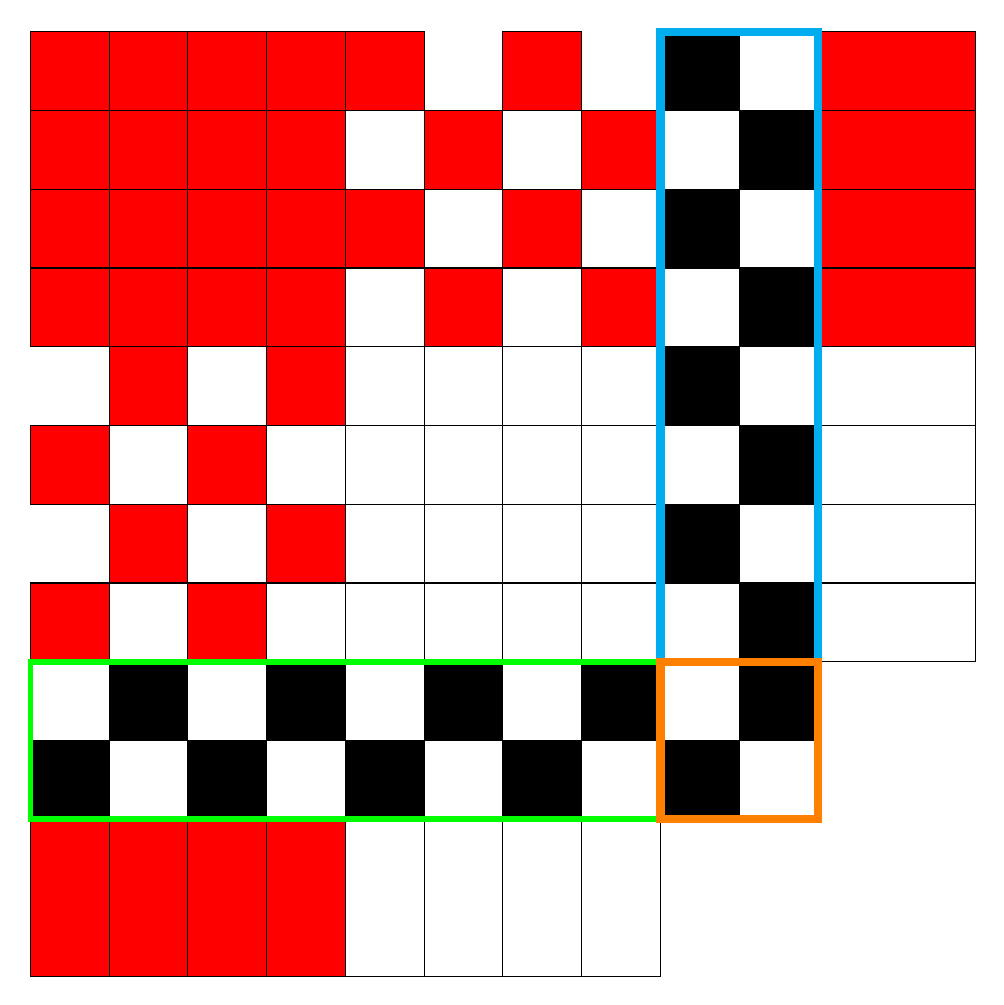
\begin{tikzpicture}
\foreach \x in {0,...,3} {
\foreach \y in {0,...,3} {
 \draw[fill=red] ({\x},{\y}) --  ++(1,0) -- ++(0,-1) -- ++ (-1,0) -- cycle;
 \draw[fill=white] ({\x+4},{\y-4}) --  ++(1,0) -- ++(0,-1) -- ++ (-1,0) -- cycle;
}
}
\foreach \x in {0,2} {
\foreach \y in {0,2} {
 \draw[fill=red] ({\x+4},{\y+1}) --  ++(1,0) -- ++(0,-1) -- ++ (-1,0) -- cycle;
 \draw[fill=red] ({\x+4+1},{\y+1-1}) --  ++(1,0) -- ++(0,-1) -- ++ (-1,0) -- cycle;
 \draw[fill=red] ({\x+1},{\y+1-4}) --  ++(1,0) -- ++(0,-1) -- ++ (-1,0) -- cycle;
 \draw[fill=red] ({\x},{\y+1-5}) --  ++(1,0) -- ++(0,-1) -- ++ (-1,0) -- cycle;
}
}
\foreach \y in {0,2,4,6}{
 \draw[fill=black] ({8},{\y-3}) --  ++(1,0) -- ++(0,-1) -- ++ (-1,0) -- cycle;
 \draw[fill=black] ({9},{\y-4}) --  ++(1,0) -- ++(0,-1) -- ++ (-1,0) -- cycle;
 \draw[fill=black] ({\y+1},-5) --  ++(1,0) -- ++(0,-1) -- ++ (-1,0) -- cycle;
 \draw[fill=black] ({\y},-6) --  ++(1,0) -- ++(0,-1) -- ++ (-1,0) -- cycle;
}

\foreach \y in {0,1,2,3}{
 \draw[fill=red] ({10},{-\y+3}) --  ++(2,0) -- ++(0,-1) -- ++ (-2,0) -- cycle;
 \draw[fill=white] ({10},{-\y-1}) --  ++(2,0) -- ++(0,-1) -- ++ (-2,0) -- cycle;
}

\foreach \x in {0,1,2,3}{
 \draw[fill=red] ({\x},-7) --  ++(1,0) -- ++(0,-2) -- ++ (-1,0) -- cycle;
 \draw[fill=white] ({\x+4},-7) --  ++(1,0) -- ++(0,-2) -- ++ (-1,0) -- cycle;
}

 \draw[fill=black] (9,-5) --  ++(1,0) -- ++(0,-1) -- ++ (-1,0) -- cycle;
 \draw[fill=black] (8,-6) --  ++(1,0) -- ++(0,-1) -- ++ (-1,0) -- cycle;

 \draw[green, line width=2] (0,-5) -- ++(8,0) -- ++(0,-2) -- ++(-8,0) -- cycle;
 \draw[cyan, line width=3] (8,3) -- ++(2,0) -- ++(0,-8) -- ++(-2,0) -- cycle;
 \draw[orange, line width=3] (8,-5) -- ++(2,0) -- ++(0,-2) -- ++(-2,0) -- cycle;
\end{tikzpicture}

\end{document}